%!TEX root = paper.tex

In this section, we first discuss the future resolution time prediction problem studied in this paper and then describe DeepER, a deep learning based system that predicts future resolution time based on past data.  



\subsection{Problem Statement}
Our aim is to design a system that accurately predicts future resolution times of incidents from historical data. For this purpose, we cast the problem as a time series prediction problem.  We consider a sequence of $n$ events with resolution times X = {$x_1$ , $x_2$ ..... $x_n$}, and predict the resolution time of the next $k$ events Y={ $y_{1}$, $y_{2}$, ..... $y_{k}$}.  What makes this problem challenging and different from classic time series prediction problems is that though these events occur chronologically, the actual time elapsed between two consecutive events varies. This is because each event corresponds to an emergency (i.e., unplanned)  and thus the time when it occurs is completely random. Hence, in some cases one may have considerable time between two consecutive events, whereas in other cases multiple events can occur in a short duration of time. Therefore, our goal is to design a flexible model that examines the resolution time of a sequence of prior events and predicts the resolution time of future events and does not depend on the actual time frame in which the events occurred.


%and then explain the implementation details including hyperparameter selection.

%Figure \ref{fig:preprocessing} shows the system architecture of DeepER. As discussed in the previous section, the data is separated into four datasets based on the incident type --- \textit{Fire}, Law, Structural and Utility. We run our model on these four datasets to get future response time predictions.

%\begin{figure}[!ht]
%    \centering
%       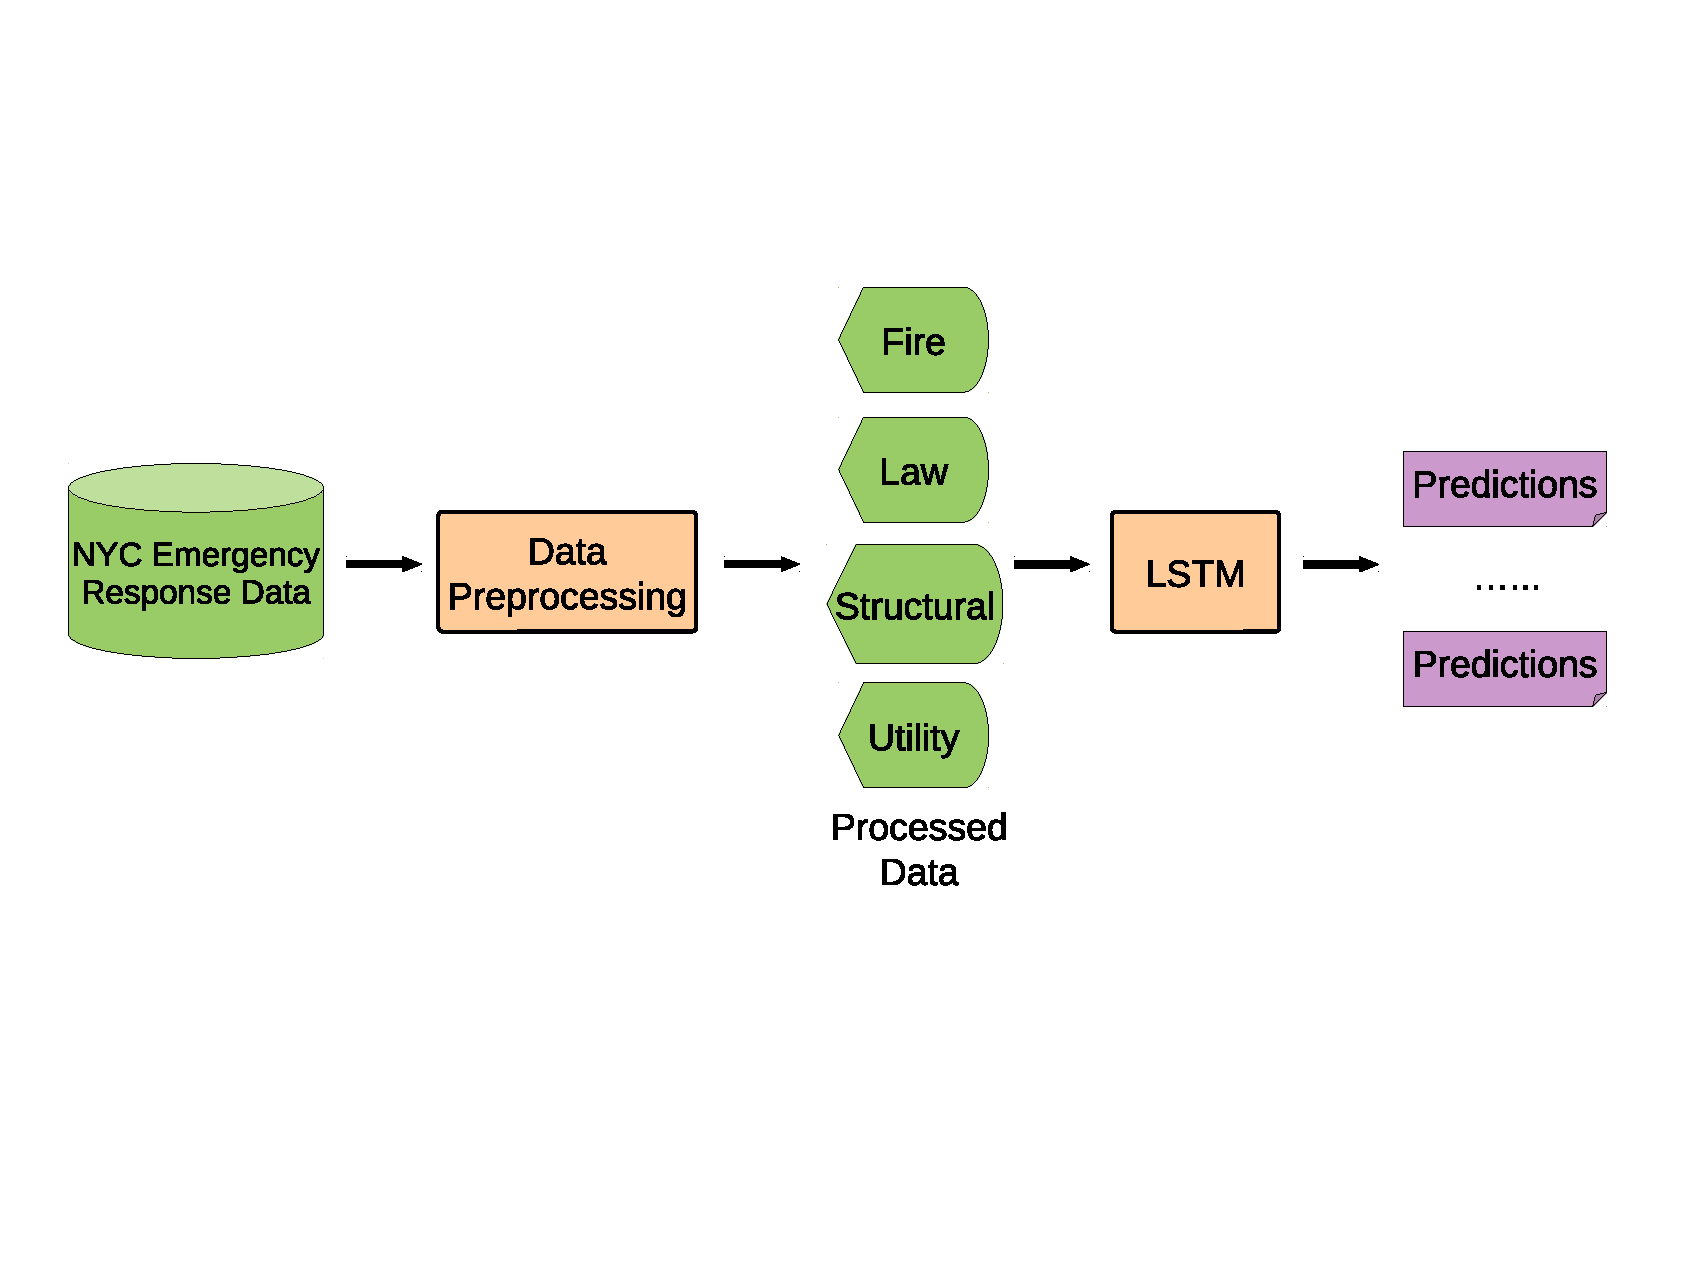
\includegraphics[trim=10 90 10 50,clip,width=1.0\linewidth]{Figures/Model/System}
%       \caption{Architecture}
%  \label{fig:architecture} 
%\end{figure}
%[trim=10 90 10 50,clip,width=1.0\linewidth]{


\begin{figure*}[!ht]
    \centering
       \includegraphics[trim=10 270 10 100,clip,scale = 0.37]{Figures/Model/preprocessing} %width=1.0\linewidth]
       \caption{DeepER System Overview}
  \label{fig:system} 
  \vspace{-3mm}
\end{figure*}



\subsection{DeepER System Details}

In this subsection, we describe DeepER, a sequence-to-sequence based encoder-decoder model that considers the resolution times of  a sequence of prior events to predict the resolution time of future events.   
Figure \ref{fig:system} provides an overview of the DeepER system. \textcolor{blue}{DeepER consists of data preprocessing block that splits the data by incidents and replaces  the outlier and missing values according to the steps outlined in Section \ref{Data:Preprocessing}. The system then splits the data into training, validation, and test (details in Section \ref{sec:implementation}) and then provides it as input to the deep learning model that uses them to generate the predictions.}

%DeepER consists of data preprocessing block that splits the data by incidents and years. The system then splits the data into training, validation, and test (details in Section \ref{sec:implementation}) and replaces  the outlier and missing values with valid points from the training set, according to the steps outlined in Section \ref{Data:Preprocessing}. Finally, the sets are provided as input to the deep learning model that uses them to generate the predictions.


\subsubsection{Sequence-to-Sequence Models}
Before delving into the system details, we discuss the appropriateness of sequence-to-sequence models for the emergency resolution time prediction problem studied here. In comparison to classic statistical regression models, sequence-to-sequence models are  better suited for this problem  as they map entire input sequences to output sequences and do not just  focus on capturing simple trends in the data. Additionally, as the points in the dataset are not  equally spaced in time and the events lack a seasonal and periodic behavioral pattern, we design deep learning based sequence-to-sequence models because such models are capable of learning the underlying dependencies and correlations in the data using an interconnected neural network architecture during the training phase and are especially useful when the dependencies are not apparent and cannot be easily defined. The trained model  leverages this knowledge to make accurate predictions at test time by considering the current input sequence.


\begin{figure}[!ht]
    \centering
       \includegraphics[trim=80 50 10 50,clip,width=1.0\linewidth]{Figures/Model/RNN}
       \caption{Encoder-decoder based RNN}
  \label{fig:RNN} 
\vspace{-3mm}
\end{figure}

\subsubsection{Encoder-decoder based RNN Model}
DeepER consists of two components, an encoder and a decoder as shown in Figure \ref{fig:RNN}. Both the encoder and the decoder comprise of recurrent neural networks (RNN). An RNN is a network of neural nodes that are arranged in layers.  Internally, the RNN has a hidden state $h_t$ that is updated at each time step $t$ using the input $x_t$ and the previous hidden state $h_{t-1}$.    At each time step $t$, the hidden state of the RNN is given by,
\begin{align}
\label{eqn:rnn}
h_t = \phi(h_{t-1}, x_t)
\end{align}
where, $\phi$ is any non-linear activation function and $1$ $\leq$ $t$ $\leq$ $n$.

As we can observe from Figure \ref{fig:RNN}, the encoder takes an input sequence $x_1$, $x_2$, ...., $x_n$ that corresponds to the resolution time of events for the last   $n$ time steps. The encoder then generates a hidden encoded vector $C$. After the entire input has been processed, the summary $C$ is provided as input to the decoder. The decoder then  generates $\hat{y}_1$, $\hat{y}_2$, ...., $\hat{y}_k$, the predicted resolution times for the future $k$ events. \textcolor{blue}{The loss function used is the sigmoid activation function and it is applied to the output of the decoder. This ensures that the predicted values are in the [0-1] range that are later inversely transformed to the original values.}

The basic cell structure used in the encoder is LSTM that captures the important dependencies in the data. LSTM cells also possess the ability to `forget' that enables them to overcome well-known vanishing/exploding gradient. To achieve this an LSTM cell has three main gates---input, output, and forget. The input gate receives the pertinent information in the current step and the output gate determines the hidden state for the next step. The forget gate is responsible for discarding unimportant information so that the model can capture the relevant long-term dependencies. We refer the reader to \cite{cho2014learning, sutskever2014sequence} for additional details.


\section{Implementation Details}
\label{sec:implementation}

In this section, we discuss implementation details regarding training, validation, and testing as well as important design   decisions (e.g.,  hyper-parameter selection).



From our discussion in the Section  \ref{Data:Preprocessing}, we observe that missing points and outliers are not spread uniformly throughout the duration of the dataset. Additionally, the entire duration of the dataset is approximately nine years and therefore, we observe gradual changes in the average resolution times of events for the same incident type. We attribute these variations to possible changes adopted by  the different emergency management agencies. These issues inherent to the dataset necessitate some important design decisions. As the underlying characteristics of the data change over time, if we adopt a simple approach and split the data chronologically into training and test, then we will end up training solely on the data for the initial few years and testing on the last few years. This is unlikely to provide good performance because the distribution of the test data sequences are  different from the distribution of the training sequences. Hence, we adopt a more careful approach where we ensure representation of data from each year in training, validation, and test datasets. 


\begin{table}[!ht]
\centering
\resizebox{\columnwidth}{!}{
\begin{tabular}{|c|c|c|c|}%|M{1.8cm}|M{1.8cm}|M{1.8cm}|M{1.8cm}|M{1.8cm}|M{1.8cm}|M{1.8cm}|}
\hline
\textbf{Sequence Length} &\textbf{Learning Rate} & \textbf{Units in Hidden Layer}\\\hline
10-3	&0.01	&10	\\\hline
10-3	&0.001	&50	\\\hline
10-3	&0.0001	&100\\\hline
15-5	&0.01	&10	\\\hline
15-5	&0.001	&50	\\\hline
15-5	&0.0001	&100\\\hline

\end{tabular}
}
\vspace{3mm}
\caption{Hypararameter combinations for experiments}
\label{tab:hyperparameter}
\end{table}


To do so, we divide the entire dataset into eight periods: seven periods of one year each and one period of approximately one and half year, approximately. We split each of these years in training, validation, and test sets following the usual percentages of 50\%, 25\%, and 25\%, respectively.  This ensures that the training, validation, and test sets contains data from all the years. Additionally, to remove any form of seasonal dependencies that may exist in the dataset, we permute the split order of training, validation and test within each year.  Such permutation ensures that the training, validation, and test data contain samples from all months of the year; in the absence of such reordering the training data will be confined to primarily the first few months, the validation confined to the middle months, and test containing data from the last few months of each year. In addition to helping in achieving good prediction performance across the entire duration of the dataset across the years, this important pre-processing step also makes our model more readily extensible to real-world deployment as the model is trained on the different variations that may be present in the data.



%%%%Figures from results section - placed here for positioning

\begin{figure*}[!ht]
    \centering
%  \subfloat[Fire]{%
%       \includegraphics[scale=0.30]{Figures/10_3/Dist/Fire_main_mae_5}
%       }
%  \subfloat[Law]{%
%       \includegraphics[scale=0.30]{Figures/10_3/Dist/Law_main_mae_6}
%       }
%  \subfloat[Structural]{%
%       \includegraphics[scale=0.30]{Figures/10_3/Dist/Structural_main_mae_7}
%       }

  \subfloat[Fire]{%
       \includegraphics[scale=0.27]{Figures/15_5/Dist/Fire_main_mae_5}
       \label{3a}}
  \subfloat[Law]{%
       \includegraphics[scale=0.27]{Figures/15_5/Dist/Law_main_mae_6}
       \label{3b}}
  \subfloat[Structural]{%
       \includegraphics[scale=0.27]{Figures/15_5/Dist/Structural_main_mae_7}
       \label{3c}}
\caption{MAE Results for the 15-5 setting}
  \label{fig:qual_mae} 
  \vspace{-3mm}
\end{figure*}

\begin{figure*}[!ht]
    \centering
%  \subfloat[Fire]{%
%       \includegraphics[scale=0.32]{Figures/10_3/Dist/Fire_main_rmse_5}
%       \label{4c}}
%  \subfloat[Law]{%
%       \includegraphics[scale=0.32]{Figures/10_3/Dist/Law_main_rmse_6}
%       \label{4d}}
%  \subfloat[Structural]{%
%       \includegraphics[scale=0.32]{Figures/10_3/Dist/Structural_main_rmse_7}
%       \label{4d}}

  \subfloat[Fire]{%
       \includegraphics[scale=0.27]{Figures/15_5/Dist/Fire_main_rmse_5}
       \label{4c}}
  \subfloat[Law]{%
       \includegraphics[scale=0.27]{Figures/15_5/Dist/Law_main_rmse_6}
       \label{4d}}
  \subfloat[Structural]{%
       \includegraphics[scale=0.27]{Figures/15_5/Dist/Structural_main_rmse_7}
       \label{4d}}  
  \caption{RMSE Results for the 15-5 setting}
  \label{fig:qual_rmse} 
  \vspace{-3mm}
\end{figure*}

 
%Thus, instead of removing them, we replace the invalid points with the valid points (response times less than quantile 90) from the training set. 



\subsection{Training, Validation, and Testing}
\label{sec:train}

We use Pytorch to implement the deep learning model.   We train our models on a Linux machine with 8-core Intel i7 processor and 64 GB RAM.
%For training our models, we leverage the shared high performance computing cluster available at our university. Using this cluster, we are able to execute multiple experiments in parallel. Each experiment is allocated 4 cores and 4 GB of RAM. %We use the response times for past $m$ events to predict the response times for future $k$ events. %As mentioned before, we split the dataset in 50\% for training, 25\% for validation and 25\% for testing. 
We use a sliding window approach with a stride of 1 to transform the time series into instances of sequences of length $n$ and prediction of length $k$. We use unguided training as the training methodology.  In this approach, the previous predicted output is used by the decoder as an input to the next step of the decoder during both training and test. Unguided approach is likely to provide better results at test time because it allows greater exploration of the state space during training. The loss function used to guide the training is the mean squared error.
% CONFIRM: We use L2 regularization in our model to avoid overfitting.

During the training phase, we experimented with various hyperparameters and then finally decided upon 6 hyperparameter combinations that are best suited for our dataset  (Table \ref{tab:hyperparameter}).  A sequence length of 10-3  in Table \ref{tab:hyperparameter} means that the model takes 10 points are input and predicts 3 points into the future. For each hyperparameter combination, we iterate over 100,000 epochs, saving the state of the model after every 5000 iterations. We then select the particular model combination that provides the best performance on the validation set.  

For quantifying the best performance, we do not simply pick the model with the lowest loss.  Such an approach usually works well when the data has overall less variation and exhibits seasonality. However, in our dataset,  events occur at random times and are of varying intensity (as each event is an emergency), thus resulting in higher variation among the values. \textcolor{blue}{This makes our dataset challenging to predict close to the mean value}. Therefore, in addition to the loss function, we also consider another heuristic, the magnitude of the standard deviation among the predictions on the validation set, to select the best model. This approach ensures that the trained model provides superior quantitative and qualitative performance. Additionally, testing on a validation set and selecting from the myriad of combinations  ensures  that we do not overfit the model to the training dataset. 






%but also the state of the model in which a minimum average standard deviation, among the steps of all predictions, is reached. %, which gives an intuition of the values that are not peaks or where most of the instances lie. 

%we observe that because of the
%We define this criteria in order to ensure our model reaches some variations and does not pick a similar value for all predictions, leading to a close-to-flat line. This minimum value is the quantile 90. We report results evaluating the best model on the test set. 

%We will make available the code for the model and the preprocessing step.
%We experiment with different number of hyperparameters like stacked layers, hidden units, learning rate and number of epochs. We observe that 1 or 2 stacked layers, 5 or 10 hidden units, initial learning rate of 0.01 and the number of epochs ranging between 5000 and 70000 give the best results depending on the incident type. We use exponential decay as the learning rate schedule in our experiments. We augment the model with a feature `sub incident type' in order to improve predictions.

%Figure \ref{fig:preprocessing} shows all the steps in the preprocessing phase. First, we group the dataset by the incident type and then apply the preprocessing steps outlined in Section \ref{Data:Preprocessing}. We then split the dataset into training, validation and test. We then apply the MinMax scale function and transform the dataset into sequences. Such a transformation ensures that all values are in the [0-1] range and is more amiable for manipulation by DeepER. When we evaluate the performance of the model we reapply the transformation to obtain the actual values.


%We calculate some thresholds to replace invalid points. Later applied the MinMax scale function and transform the dataset into sequence instances. Finally, the splits percentages are no exactly the original 50\%, 25\% and 25\% but values near to these ones. This happens due to the cuts among years that, in some cases, trunc the continuation of time steps invalidating instances of lengths $m+k$. We observe that preprocessing does not affect too much the statistics values for Law because it already has smaller values compared to the other incident types. However, the statistics values for Fire and Structural show more perceptible reduction. Additionally, the outlier values before preprocessing, cut off for visualization purposes to 8000 minutes, are much larger than the values after preprocessing.




